\section{Результаты использования программного средства}
\label{sec:results}

В данном разделе будут описаны результаты, полученные с помощью программного средства,
основанного на разработанной модели паники.

Большинство экспериментов было поставлено в режиме эвакуации, так как данный режим
является наиболее интересным в рамках исследования моделей паники.

Для проведения экспериментов была создана схема сооружения, приближенная к реальному офисному зданию.

\begin{figure}[ht!]
  \centering
  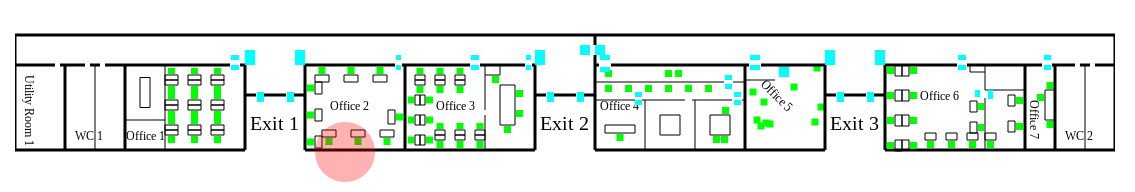
\includegraphics[width=\linewidth]{masters_office_scene}
  \caption{Схема сооружения, используемая в большинстве опытов}
  \label{sec:results:office_scene}
\end{figure}

На рисунке~\ref{sec:results:office_scene} изображена упомянутая схема сооружения.
Толстыми черными линиями обозначены стены, тонкими черными линиями "--- предметы мебели и внутриофисные перегородки.
Зеленые области соответствуют начальному положению людей в офисе.
Бирюзовые области задают промежуточные точки, которые люди должны посетить на пути к выходу.
Шесть бирюзовых областей рядом с надписями Exit 1, 2 и 3 являются конечной целью всех людей.
Розовый круг во втором офисе представляет источник паники.

\subsection{Влияние случайных флуктуаций на время эвакуации}
\label{sec:results:fluctuation}

Для проведения данного эксперимента была временно убрана зависимость вероятности возникновения и силы флуктуаций от уровня паники пешехода "---
уровень паники всегда считался равным 1.0, но только для силы случайных флуктуаций.

Сначала было произведено несколько контрольных замеров при силе флуктуаций равном нулю.
Время эвакуации в среднем получилось около 15 секунд, с минимумом в 5 и максимумом в 30 секунд.

При увеличении силы флуктуации до трети желаемой скорости пешехода начинают проявляться первые эффекты.
Флуктуации еще не достаточны, чтобы сбить с правильного пути пешехода, однако они уже могут значительно его замедлить.
Время эвакуации в среднем увеличивается не сильно (до 16 секунд), но максимальное время увеличивается до 40-50 секунд.

При увеличении силы флуктуации до двух третей желаемой скорости пешехода эффект становится намного более заметным.
Среднее время эвакуации увеличивается до 20 секунд, максимальное время увеличивается до 50-60 секунд.

\begin{figure}[ht!]
  \centering
  \begin{subfigure}[!htb]{0.45\textwidth}
    \centering
    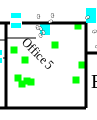
\includegraphics[scale=1.5]{masters_fluctuation_jam}
    \caption{}
  \end{subfigure}
  \begin{subfigure}[!htb]{0.45\textwidth}
    \centering
    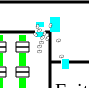
\includegraphics[scale=1.5]{masters_fluctuation_jam2}
    \caption{}
  \end{subfigure}
  \caption{Примеры пробок при большой силе флуктуации}
  \label{sec:results:fluctuation:jam}
\end{figure}

И наконец при силе флуктуации равной желаемой скорости пешехода эффект становится очень сильным.
Флуктуации достаточны, чтобы сбить пешехода с правильного пути.
Такие пешеходы сразу выбиваются из потока, пытаются идти против направления движения большинства, чем вызывают появление пробок (пример на рисунке~\ref{sec:results:fluctuation:jam}).
Среднее время эвакуации увеличивается до 40 секунд, максимальное - до 80-140 секунд.

Таким образом, случайные флуктуации (представляющие случайные иррациональные решения пешехода) оказывают строго негативное влияние на время эвакуации.
Механизм, увеличивающий время эвакуации, очевиден "--- флуктуации мешают пешеходам двигаться к своей цели кратчайшим путем,
что приводит к более длинному пути к выходу, а следовательно и к более длительной эвакуации.
При экстремальной силе флуктуаций они вызывают пробки из-за несовпадения направления движения некоторых людей в потоке с самим потоком.
Данный эффект очень сильно увеличивает время эвакуации.

\subsection{Влияние уменьшения силы отталкивания и использования большой силы физического контакта}
\label{sec:results:repulsion}

Как и в предыдущем разделе, воспользуемся возможностью вручную контролировать уровень паники для силы отталкивания.
Проведем эксперимент с обычной силой отталкивания (уровень паники равен нулю), а потом будем постепенно уменьшать силу отталкивания (увеличивать уровень паники)
и наблюдать за возможными эффектами.

В данном эксперименте были получены довольно интересные результаты: изменение силы отталкивания практически никак не влияет на время эвакуации.
Даже при полностью отсутствующей силе отталкивания (при использовании лишь физических сил контакта) время эвакуации не меняется.

Таким образом, выбранная модель физического контакта не способна адекватно обработать сложные физические взаимодействия.
Модели не хватает учета инерции и последствий столкновений, однако разработка такой улучшенной модели выходит за рамки данной работы.

\subsection{Влияние силы <<стадного поведения>>}
\label{sec:results:herding}

Проведем следующий эксперимент: будем варьировать коэффициент учета силы <<стадного поведения>> в итоговой силе, действующей на пешехода.

К сожалению, результат оказался аналогичен предыдущему разделу "---
сила <<стадного поведения>> очень слабо влияет на итоговое время эвакуации при разумном значении коэффициента.

Если выставить слишком высокое значение коэффициента, итоговое время эвакуации увеличиться, однако данный эффект имеет мало общего с реальностью.
При высоком значении коэффициента определенные пешеходы <<подхватываются>> потоком и следуют за ним некоторое время.
Однако потом такой пешеход все равно возвращается назад, так как следуя за потоком он пропустил некоторые контрольные точки на своем пути (пример на рисунке~\ref{sec:results:herding:returning}).

\begin{figure}[ht!]
  \centering
  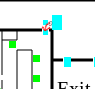
\includegraphics[scale=1.5]{masters_herding_returning}
  \caption{Примеры пешехода, возвращающегося назад после следования за потоком (стрелкой отмечено направление движения)}
  \label{sec:results:herding:returning}
\end{figure}

Таким образом, описанная проблема является не проблемой модели паники, а проблемой реализованного программного средства.
Для полноценного исследования влияния силы <<стадного поведения>> программное средство должно также реализовывать модель целеполагания пешехода.

Эффекты данной силы должны проявляться при ситуации, когда пешеход не знает текущего направления к выходу.
В таком случае данная сила должна помочь пешеходам выбрать одно направление.
Однако при слишком высоком влиянии данной силы люди могут следовать за кем-то,
кто тоже не знает направления к выходу, тем самым увеличивая время эвакуации.

Разработанное же программное средство в целях упрощения приняло, что каждый пешеход всегда знает направление к выходу.
Поэтому для исследования влияния данной силы требуется разработка модели поиска выхода для каждого пешехода, учитывающей
возможность того, что некоторые пешеходы знают направление к выходу, а некоторые "--- нет.

\subsection{Проявление макроскопических эффектов}
\label{sec:results:macro}

При разработке модели было высказано предположение, что некоторые макроскопические эффекты
(например, скопление людей в дверях и на выходе) должны сами проявиться при реализации простых сил модели.

Действительно, разработанная модель демонстрирует возникновение макроскопических эффектов.
Самым заметным среди них можно назвать эффект возникновения устойчивых потоков людей (рисунок~\ref{sec:results:macro:flow}).
Также возникают эффекты скопления людей в дверях (рисунок~\ref{sec:results:macro:jam}) и
нескоординированности прохода через узкие места.

\begin{figure}[ht!]
  \centering
  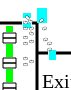
\includegraphics[scale=1.5]{masters_macro_flow}
  \caption{Пример образования устойчивого потока людей}
  \label{sec:results:macro:flow}
\end{figure}

\begin{figure}[ht!]
  \centering
  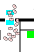
\includegraphics[scale=1.5]{masters_macro_jam}
  \caption{Пример образования скопления людей в дверях}
  \label{sec:results:macro:jam}
\end{figure}

Последний эффект очень специфичен, так как должен наблюдаться только при условии,
что через одно узкое место пешеходы пытаются пройти в разных направлениях.
В сценарии эвакуации данное условие никогда не должно наблюдаться, однако в некоторых случаях
(при очень сильной силе флуктуаций, либо иногда при неудачном стечении обстоятельств и сильном влиянии
<<стадного>> поведения) такой эффект возникает и в разрабатываемой модели.

Рисунок с примером данного эффекта уже был представлен в разделе~\ref{sec:results:fluctuation}, рисунок~\ref{sec:results:fluctuation:jam}.
В данном редком случае два пешехода пытаются пройти вправо, а два "--- влево.
В результате нескоординированности это занимает у них значительное количество времени.


\subsection{Модель распространения паники}
\label{sec:results:panic_spread}

В разработанном программном средстве была реализована модель распространения паники.
Для ее тестирования воспользуемся другой, более простой схемой сооружения (рисунок~\ref{sec:results:panic_spread:scene}).
На данной схеме сооружения будет единственный поток пешеходов снизу вверх. Некоторая часть этого потока попадет в зону источника паники.
При правильно подобранных коэффициентах, уровень паники во всем потоке должен возрасти до максимума.

\begin{figure}[ht!]
  \centering
  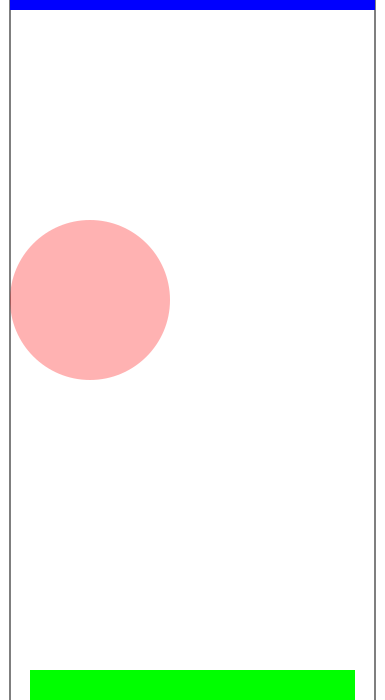
\includegraphics[scale=0.5]{masters_panic_scene}
  \caption{Схема сооружения для тестирования паники}
  \label{sec:results:panic_spread:scene}
\end{figure}

Подбирая значения коэффициентов $k_{ipl}$, $k_{spl}$, $k_{dpl}$ добьемся вышеобозначенной цели.
На рисунке~\ref{sec:results:panic_spread:ks} представлены три этапа распространения паники:

\begin{itemize}
  \item начальный этап: первые пешеходы только получили максимальный уровень паники от источника паники;
  \item промежуточный этап: паника распространяется по пешеходам;
  \item конечный этап: все пешеходы имеют максимальный уровень паники, каждый новый пешеход также сразу получает максимальный уровень паники.
\end{itemize}

\begin{figure}[ht!]
  \centering
  \begin{subfigure}[!htb]{0.3\textwidth}
    \centering
    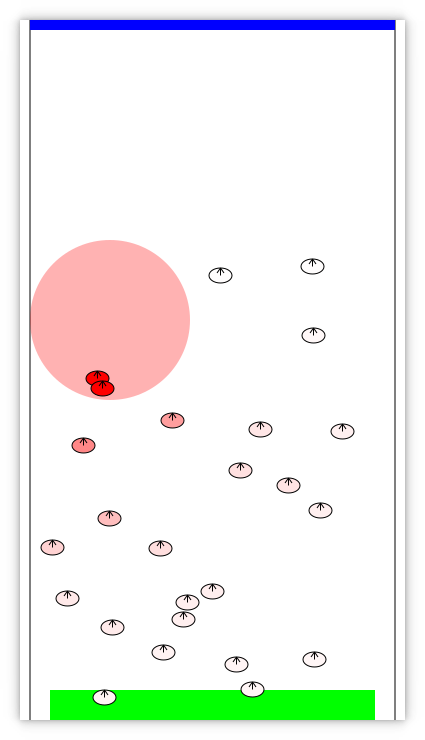
\includegraphics[scale=0.5]{masters_spread_init}
    \caption{}
  \end{subfigure}
  \begin{subfigure}[!htb]{0.3\textwidth}
    \centering
    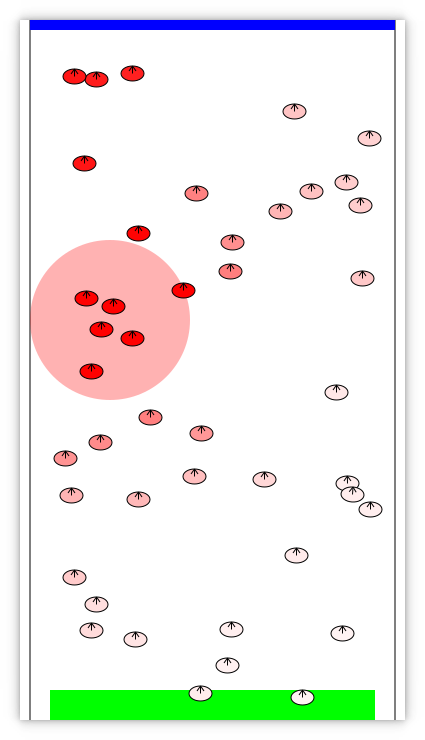
\includegraphics[scale=0.5]{masters_spread_middle}
    \caption{}
  \end{subfigure}
  \begin{subfigure}[!htb]{0.3\textwidth}
    \centering
    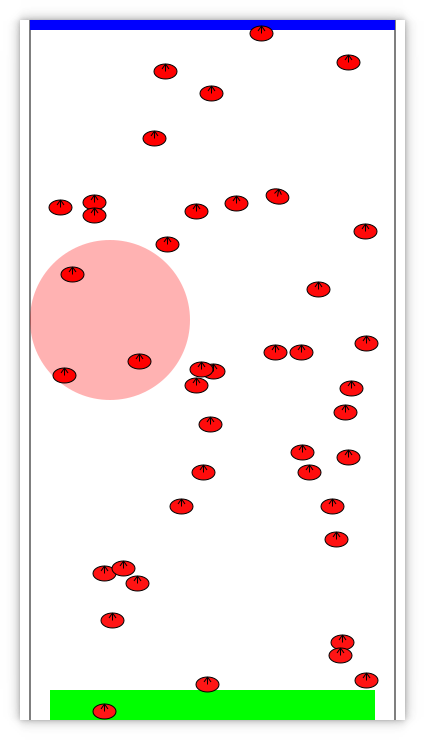
\includegraphics[scale=0.5]{masters_spread_finish}
    \caption{}
  \end{subfigure}
  \caption{Этапы распространения паники: а "--- начальный, б "--- промежуточный, в "--- конечный}
  \label{sec:results:panic_spread:ks}
\end{figure}

Такой результат был достигнут при значениях коэффициентов $k_{ipl} = 1.0$, $k_{spl} = 1.0$, $k_{dpl}$ равный утере примерно 20\% уровня паники в секунду.

Стоит отметить, что данные значения коэффициентов хорошо работают и в более сложных ситуациях, например на тестовой схеме сооружения офиса.
На рисунке \ref{sec:results:panic_spread:office} представлен пример распространения паники в офисе.

\begin{figure}[ht!]
  \centering
  \begin{subfigure}[!htb]{1.0\textwidth}
    \centering
    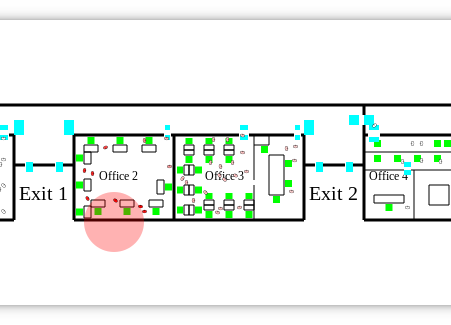
\includegraphics[width=\linewidth]{masters_spread_complex_init}
    \caption{}
  \end{subfigure}
  \begin{subfigure}[!htb]{1.0\textwidth}
    \centering
    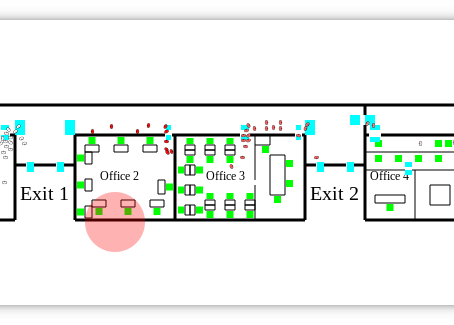
\includegraphics[width=\linewidth]{masters_spread_complex_finish}
    \caption{}
  \end{subfigure}
  \caption{Этапы распространения паники в сложной схеме сооружения: а "--- начальный, б "--- конечный}
  \label{sec:results:panic_spread:office}
\end{figure}

Можно сделать вывод, что разработанная модель распространения паники выглядит реалистично.
К сожалению, такое абстрактное понятие как <<уровень паники>> тяжело измерить,
а следовательно доказать реалистичность выбранной модели также тяжело.
